\chapter{Results}
\label{sec:results}
The most interesting questions regarding \emph{HELM} are
\begin{itemize}
	\item How well does \emph{HELM} work compared to the iterative methods?
	\item Is \emph{HELM} able to calculate large scale power nets, for which the iterative methods do not converge?
\end{itemize}
To answer these questions I have run several experiments. The ones related to the first question can be found in \secinref{comparison_algorithms}. To answer the second question I will describe in \secinref{large_scale_power nets} the results of running \emph{HELM} on a large scale power net with a few thousand nodes.

\section{Comparison of the Load-flow Algorithms}
\label{sec:comparison_algorithms}

\begin{table}
	\small
	\begin{tabularx}{\textwidth}{|X|p{0.9cm}|p{0.8cm}|p{0.9cm}|p{0.8cm}|p{1.3cm}|}
		\hline
		method & \rotatebox[origin=c]{90}{target precision} & \rotatebox[origin=c]{90}{maximum iterations} & \rotatebox[origin=c]{90}{datatype size} & \rotatebox[origin=c]{90}{maximum coefficients} & \rotatebox[origin=c]{90}{solver} \\ \hline
		\emph{Current Iteration} & 1e-5 & 100 & & & iterative \\ \hline
		\emph{Newton-Raphson} & 1e-5 & 100 & & & iterative \\ \hline
		\emph{HELM} 64 Bit & 1e-5 & & 64 & 50 & iterative \\ \hline
		\emph{HELM} 200 Bit & 1e-5 & & 200 & 100 & iterative \\ \hline
		\emph{HELM} 64 Bit with \emph{Current \mbox{Iteration}} & 1e-5 & 100 & 64 & 50 & iterative \\ \hline
	\end{tabularx}
	\caption{Algorithm parameters for the runtime and accuracy comparison}
	\label{tab:comparison_parameter}
\end{table}

\begin{table}
	\small
	\begin{tabularx}{\textwidth}{|X|p{0.9cm}|p{0.8cm}|p{0.9cm}|p{0.8cm}|p{1.3cm}|}
		\hline
		method & \rotatebox[origin=c]{90}{target precision} & \rotatebox[origin=c]{90}{maximum iterations} & \rotatebox[origin=c]{90}{datatype size} & \rotatebox[origin=c]{90}{maximum coefficients} & \rotatebox[origin=c]{90}{solver} \\ \hline
		\emph{HELM}, 64 Bit, iterative & 1e-10 & & 64 & 50 & iterative \\ \hline
		\emph{HELM}, 64 Bit, LU & 1e-10 & & 64 & 50 & LU \\ \hline
		\emph{HELM} with \mbox{\emph{Current Iteration}}, 64 Bit, LU & 1e-10 & 100 & 64 & 50 & LU \\ \hline
		\emph{HELM}, 100 Bit, LU & 1e-10 & & 100 & 70 & LU \\ \hline
		\emph{HELM}, 200 Bit, LU & 1e-10 & & 200 & 100 & LU \\ \hline
		\emph{HELM}, 1000 Bit, LU & 1e-10 & & 1000 & 200 & LU \\ \hline
		\emph{HELM}, 10000 Bit, LU & 1e-10 & & 10000 & 300 & LU \\ \hline
		\emph{Current Iteration}, iterative & 1e-10 & 100 & & & iterative \\ \hline
		\emph{Current Iteration}, LU & 1e-10 & 100 & & & LU \\ \hline
		\emph{Newton-Raphson}, iterative & 1e-10 & 100 & & & iterative \\ \hline
		\emph{Newton-Raphson}, LU & 1e-10 & 100 & & & LU \\ \hline
		\emph{Newton-Raphson}, SINCAL & 1e-10 & 100 & & & \\ \hline
	\end{tabularx}
	\caption{Algorithm parameters for the convergence comparison}
	\label{tab:comparison2_parameter}
\end{table}

\begin{figure}
	\centering
	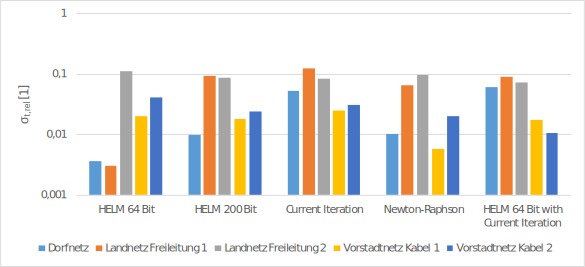
\includegraphics[scale=0.7]{figures/comparison_deviation}
	\caption[Comparison, relative standard deviation of runtime]{Relative standard deviation of the runtime of the algorithms}
	\label{fig:comparison_deviation}
\end{figure}

To compare the different load-flow algorithms I used the sample nets of the Institute and compared the algorithms then regarding their runtime and accuracy. I have already considered the improved convergence behaviour in \secinref{implementation_helm}, but I will show additional results regarding this aspect in this chapter.

The selected algorithms for this comparison cover nearly the whole possible spectrum which is implemented in the tool, including the usage of \emph{HELM} to calculate seed values for an iterative method. This special application of \emph{HELM} is represented by the algorithm \emph{HELM} with \emph{Current Iteration}.

The parameters for the algorithms in the accuracy and runtime comparison can be found in \tabinref{comparison_parameter}, the settings for the convergence border tests are in \tabinref{comparison2_parameter}.

To eliminate influences by other processes or the garbage collection on the runtime, I ran the calculations five times. The resulting runtimes did not vary much considering the relative standard deviations \figref{comparison_deviation}.

\subsection{Runtime}

\begin{figure}
	\centering
	
\includegraphics[scale=0.7]{figures/comparison_runtime}
	\caption[Comparison, average runtime]{Average runtime of the algorithms for several power nets}
	\label{fig:comparison_runtime}
\end{figure}

One key point is the runtime, and this depends heavily on the implementation of not only the algorithms themselves, but also on the used tools like the library for the sparse linear algebra. Therefore, I am not able to make absolute statements here, especially because I even implemented \emph{HELM} in a different language than the other algorithms and optimized the linear algebra there.

The first important message here is that \emph{HELM} with 64 Bit is considerably fast compared to the \emph{Current Iteration} and \emph{Newton-Raphson}, as it can be seen in \figinref{comparison_runtime}. If \emph{Newton-Raphson} runs into convergence problems like in the case of the Vorstadtnetz, \emph{HELM} is even faster than this iterative approach. 

Another conclusion from these tests is that the combination of \emph{HELM} with an iterative method, for instance with the \emph{Current Iteration}, is a very handy approach. In \secinref{implementation_helm} I have already shown that this improves the convergence behaviour, but if we also take the runtime into account the combination is not really a drawback. Considering this, I recommend to use always \emph{HELM} with the \emph{Current Iteration} instead of only the latter one.

The last important message is the insufficient performance of \emph{HELM} with a datatype bigger than 64 Bit. This setting avoids that floating point operations can be executed within a few clock cycles with the integrated assembler commands and therefore deterioates the performance of the algorithm significantly. Consequently, I recommend to use \emph{HELM} with a bigger datatype only in situations where the calculation with \emph{HELM} with 64 Bit failed.

\subsection{Accuracy}

As a metric for the accuracy I used the relative power error, which is the ratio between power error and total power, both summed up absolutely:
\begin{equation}
	\epsilon_r = \frac{\sum |P_i - P_{spec,i}| + \sum |Q_i - Q_{spec,i}|}{\sum |P_{spec,i}| + \sum |Q_{spec,i}|}
\end{equation}

The accuracies of the algorithms \figref{comparison_accuracy} were all sufficient for most applications, although a difference can be seen between the pure iterative approaches and the ones with \emph{HELM}. The later ones are able to deliver more accurate results for these nets. Keeping in mind that \emph{HELM} is even as fast as the \emph{Current-Iteration}, at least in my implementation, there is no reason to use the \emph{Current Iteration} instead of \emph{HELM} or \emph{HELM} together with the \emph{Current Iteration}.

\begin{figure}
	\centering
	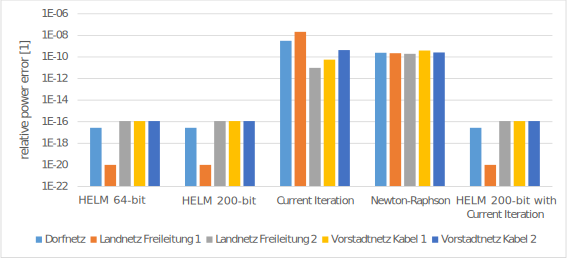
\includegraphics[scale=0.7]{figures/comparison_accuracy}
	\caption[Comparison, accuracy]{Relative power error of the algorithms}
	\label{fig:comparison_accuracy}
\end{figure}

\subsection{Convergence}

To test and compare the convergence behaviour of the different algorithms I used one of the example nets from the institute, the so-called \emph{Vorstadtnetz}. In this net I then increased the load at the most outer ends of the radial net up to that point, where the algorithm did not converge anymore. To find this convergence border more efficiently, I applied the bisection method.

The first and most obvious conclusion, which can be drawn from \figinref{comparison_convergence_border_1}, is that the iterative solver for the internal linear equation systems deteriorates the convergence behaviour of \emph{HELM} significantly. 

Secondly, at least for this special case, the implementation of \emph{Newton-Raphson} in \emph{SINCAL} has a worse convergence behaviour with these settings, compared to my implementation. But I want to make clear that this depends heavily on the settings of the algorithm, and I could only guess how the certain parameters are actually implemented in \emph{SINCAL}. Therefore, it is not really possible to draw a useful conclusion from this experiment regarding the implemention in \emph{SINCAL}.

If we zoom into this chart we get at the first step \figinref{comparison_convergence_border_2}, which reveals that \emph{HELM} in its pure form outperforms the other methods, considering the convergence behaviour. After another zoom step one can see in \figinref{comparison_convergence_border_3} that a more accurate datatype improves the convergence behaviour of \emph{HELM}, although only a few thousand watts. Additionally, such extrordinary settings effect the runtime of the algorithm significantly, as it then takes a few hours to calculate such a net, compared to only a few seconds with 64 Bit.

\begin{figure}
	\centering
	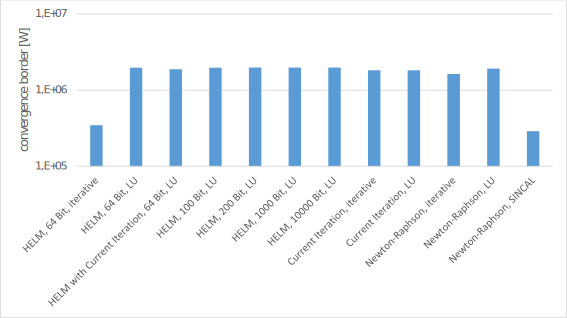
\includegraphics[scale=0.7]{figures/convergence_border_vorstadtnetz_1}
	\caption[Comparison, convergence]{Convergence border of the algorithms}
	\label{fig:comparison_convergence_border_1}
\end{figure}

\begin{figure}
	\centering
	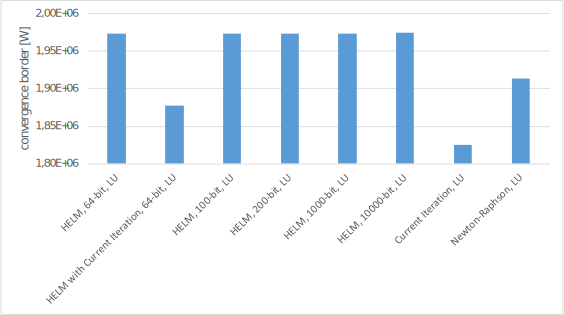
\includegraphics[scale=0.7]{figures/convergence_border_vorstadtnetz_2}
	\caption[Comparison, convergence]{Convergence border of the algorithms}
	\label{fig:comparison_convergence_border_2}
\end{figure}

\begin{figure}
	\centering
	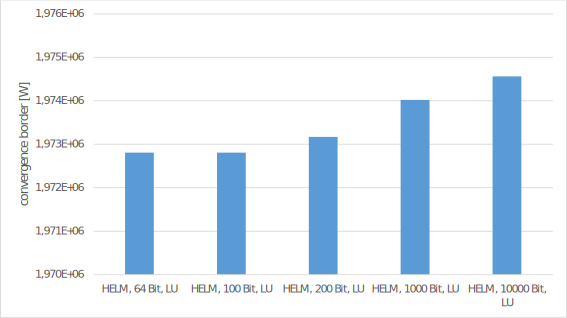
\includegraphics[scale=0.7]{figures/convergence_border_vorstadtnetz_3}
	\caption[Comparison, convergence]{Convergence border of the algorithms}
	\label{fig:comparison_convergence_border_3}
\end{figure}

\section{Calculation of Large-Scale Power Nets}
\label{sec:large_scale_power nets}
	
To evaluate \emph{HELM} in the scenario of large-scale power nets I used the power net of \emph{infra fürth}, which they kindly provided for this purpose. Due to the current limitations of \emph{HELM} I had to adapt the power net. For instance, \emph{HELM} currently does not support non-linear current controlled sources, which were used in the power net of \emph{infra fürth} for the photovoltaic installations, as well as for the generators. To circumvent this I removed all these not supported elements.

Another important thing to point out is the switching state, the version I received was configured in a way that the total net was split up into three parts. For the comparison later on I used this initial version, as well as one where these three parts were connected together. In the connected version there was then one big net with more than 50000 nodes.

As algorithms for the comparison I selected:
\begin{itemize}
	\item \emph{HELM} with a 64 Bit datatype and LU factorization
	\item \emph{Current Iteration} with an iterative solver
	\item \emph{HELM} with 64 Bit datatype and LU factorization and as second step \emph{Current Iteration} with an iterative solver
	\item \emph{PSS SINCAL} with the default configuration
\end{itemize}
Unfortunately, the library I used for the linear algebra in the iterative load-flow algorithms was not able to calculate the LU factorization at all in a reasonable amount of time. Additionally, the calculation of the Jacobian matrix was not very efficient too, due to the sparse matrix implementation. Therefore, I had to leave out my implementation of \emph{FDLF} and \emph{Newton-Raphson}, but this class of algorithms is still represented in the comparison through \emph{PSS SINCAL}.

As I implemented \emph{HELM} in \emph{C++} and optimized the LU factorization for these circumstances, I was able to select this combination for the tests. By the way, this shows that the performance of the algorithms depends heavily on the implementation of the linear algebra.

\begin{figure}
	\centering
	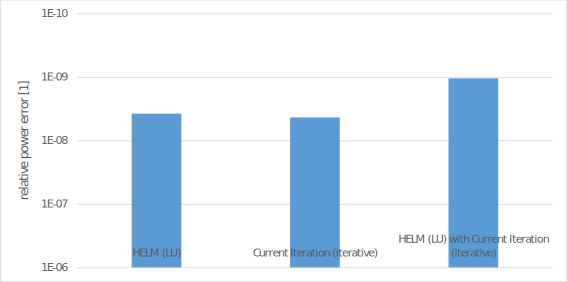
\includegraphics[scale=0.7]{figures/big_net_separate_relative_power_error}
	\caption[Comparison, \emph{infra fürth}, separate, error]{relative power error of the algorithms for the separated version of the power net of \emph{infra fürth}}
	\label{fig:big_net_separate_relative_power_error}
\end{figure}

\begin{figure}
	\centering
	\includegraphics[scale=0.7]{figures/big_net_combined_relative_power_error}
	\caption[Comparison, \emph{infra fürth}, connected, error]{relative power error of the algorithms for the connected version of the power net of \emph{infra fürth}}
	\label{fig:big_net_combined_relative_power_error}
\end{figure}

First, I would like to point out the relative power errors of the algorithms for these two versions of the power net in \figinref{big_net_separate_relative_power_error} and \figinref{big_net_combined_relative_power_error}. For most applications of a load-flow algorithm this accuracy should be sufficient.

\begin{figure}
	\centering
	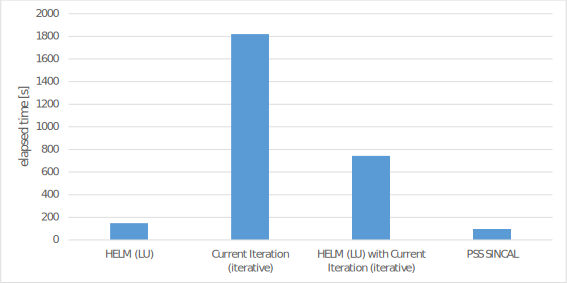
\includegraphics[scale=0.7]{figures/big_net_separate_runtime}
	\caption[Comparison, \emph{infra fürth}, separate, runtime]{runtime of the algorithms for the separated version of the power net of \emph{infra fürth}}
	\label{fig:big_net_separate_runtime}
\end{figure}

\begin{figure}
	\centering
	\includegraphics[scale=0.7]{figures/big_net_combined_runtime}
	\caption[Comparison, \emph{infra fürth}, connected, runtime]{runtime of the algorithms for the connected version of the power net of \emph{infra fürth}}
	\label{fig:big_net_combined_runtime}
\end{figure}

Second, the comparison of the runtime in \figinref{big_net_separate_runtime} and \figinref{big_net_combined_runtime} shows that \emph{HELM} is able to get close to the performance of \emph{PSS SINCAL}. Contrary, the \emph{Current Iteration} with the iterative solver for the linear equation systems is outperformed by \emph{HELM} and \emph{PSS SINCAL} by orders of magnitude. Obviously, the real game changer here is the linear algebra, as the admittance matrix has a bad condition in these scenarios.

\section{Conclusion}
In conclusion, \emph{HELM} is superior to the iterative methods, regarding the convergence behaviour. This advantage comes directly from the theoretical background, where so far only \emph{HELM} can be proven to have a perfect convergence behaviour. The only limitation which is left here is caused by the machine epsilon of the computer. Considering the runtime, \emph{HELM} can not reach the performance of for instance \emph{FDLF} if the latter one converges within only a few iterations.

In summary, there exist mainly two reasons not to use \emph{HELM}:
\begin{enumerate}
	\item The calculation has to be done fast
	\item A certain control is used in the power net, which is not yet supported by \emph{HELM}
\end{enumerate}
The first drawback here is immanent in \emph{HELM}, but the second one will be a topic for future research.

Finally, in practical applications it is handy to have a fallback in case the iterative methods do not converge.